\documentclass[11pt,a4paper]{article}

% --- Essential Packages ---
\usepackage[top=2.2cm, bottom=2.2cm, left=2.2cm, right=2.2cm]{geometry}
\usepackage{amsmath, amssymb, amsfonts, amsthm, mathtools}
\usepackage{graphicx}
\usepackage{subcaption}
\usepackage{booktabs, multirow, makecell}
\usepackage{algorithm, algpseudocode}
\usepackage{xcolor}
\usepackage{cite}
\usepackage{microtype}
\usepackage{titlesec}
\usepackage[colorlinks=true, linkcolor=blue!80!black, citecolor=blue!80!black, urlcolor=blue!80!black]{hyperref}

\linespread{1.15}

% --- Custom Section Numbering (Roman Numerals matching Vietnamese Report) ---
\renewcommand{\thesection}{\Roman{section}}
\titleformat{\section}{\large\bfseries}{\thesection.}{0.5em}{}
\titlespacing*{\section}{0pt}{14pt plus 2pt minus 2pt}{8pt plus 2pt minus 2pt}

\titleformat{\subsection}{\normalsize\bfseries}{}{0pt}{}
\titlespacing*{\subsection}{0pt}{10pt plus 2pt minus 2pt}{6pt plus 2pt minus 2pt}

\begin{document}

% --- Institutional Header & 6G Badge ---
\noindent
\begin{minipage}[t]{0.75\textwidth}
    \textbf{Posts and Telecommunications Institute of Technology (PTIT)}\\
    \textbf{Faculty of Telecommunications II}\\[0.12cm]
    \small \textbf{Email:} \texttt{nmquan3108@gmail.com}
\end{minipage}%
\hfill

\vspace{0.25cm}
\hrule height 0.8pt
\vspace{0.8cm}

% --- Document Title ---
\begin{center}
    {\LARGE \textbf{Joint Trajectory and Power Allocation Optimization\\[0.25cm]
    in SAGIN-NOMA Networks:\\[0.28cm]
    From Alternating Optimization (AO) to Real-Time Deep Reinforcement Learning (DRL)}}\\[0.6cm]
\end{center}

% --- Main Body Sections ---
\section{Executive Summary}
\label{sec:exec_summary}

This report provides a rigorous quantitative analysis of the optimization framework for Space-Air-Ground Integrated Networks empowered by Non-Orthogonal Multiple Access (SAGIN-NOMA). The core objective of this study is to minimize the total system outage probability ($P_{\text{out}}$), enhancing transmission reliability over generalized Rician fading channels while strictly ensuring the mathematical and physical feasibility of Successive Interference Cancellation (SIC). The report details a dual-hop system model (Satellite $\to$ UAV relay cluster with PRS mechanism $\to$ Two ground users), derives exact closed-form analytical expressions via the first-order Marcum-Q function, and presents two complementary optimization paradigms: (i) a numerical Alternating Optimization (AO) benchmark serving as the theoretical performance baseline; and (ii) a custom Deep Reinforcement Learning (DRL) agent based on the Actor-Critic architecture that enables online trajectory control and power allocation decisions at the millisecond scale. Simulation results, quantitative comparative analyses, and technical implementation specifications on 6G aerial platforms are thoroughly presented in this report.

\section{Introduction \& Background}
\label{sec:intro_background}

\subsection*{Background}

Space-Air-Ground Integrated Networks (SAGIN) are envisioned as a foundational infrastructure for sixth-generation (6G) wireless communications, aiming to eliminate coverage blind spots in remote areas, open oceans, mountainous regions, and disaster rescue scenarios \cite{liu2018space, zeng2019accessing}. In this architecture, satellites provide broad wide-area coverage but suffer from severe free-space path loss. The integration of Unmanned Aerial Vehicles (UAVs) acting as Decode-and-Forward (DF) relay stations helps regenerate signals, shorten transmission distances, and establish favorable line-of-sight (LoS) links \cite{wu2018joint}. When combined with power-domain Non-Orthogonal Multiple Access (NOMA), the UAV can simultaneously serve multiple terrestrial users over the same time-frequency resource block, substantially boosting spectral efficiency \cite{ding2017application}. However, the flexible mobility of the UAV necessitates stringent spatial boundary management to prevent inversions of the successive interference cancellation (SIC) decoding order, formulating a complex, non-convex non-linear optimization problem.

\subsection*{Project Objectives}

The project focuses on addressing three specific technical objectives:
\begin{enumerate}
    \item \textbf{Exact Analytical Derivation:} Establish exact closed-form analytical expressions for the outage probability (OP) of individual users and the overall system over generalized Rician fading channels via the first-order Marcum-Q function \cite{simon2005digital}, incorporating the Partial Relay Selection (PRS) scheme.
    \item \textbf{Establishment of Numerical Benchmark (AO Benchmark):} Construct an Alternating Optimization (AO) framework that decouples the joint optimization problem into trajectory optimization (using Sequential Quadratic Programming - SQP) and power allocation (using Golden Section Search) under kinematic constraints and geometric SIC boundaries.
    \item \textbf{Real-Time Control Implementation (Real-Time DRL):} Design and train a continuous Actor-Critic neural network based on the Deep Deterministic Policy Gradient (DDPG) algorithm \cite{lillicrap2015continuous} with Guided Displacement and Warm-Start Seeding, achieving an inference latency of $\approx 1.5$ ms/slot for adaptive real-time online aerial flight guidance.
\end{enumerate}

\section{Methodology \& Technical Model}
\label{sec:methodology}

\subsection*{System Overview}

The SAGIN-NOMA network system is modeled in a normalized 2D coordinate plane $(Oxz)$ with the following physical components and parameters:
\begin{itemize}
    \item \textbf{Spatio-Temporal Architecture:} A source satellite $S$ at normalized coordinates $\mathbf{q}_S = (0.0, 1.0)$ (an illustrative normalized 2D geometric model with reference scaling distance $D_0 = 125$ m); a cluster of $N_{\text{UAV}} = 3$ UAV relays flying in close formation around a nominal waypoint $\mathbf{q}_U[n]$ (the PRS mechanism selects the UAV with the highest instantaneous channel gain within the cluster); and two ground users comprising near user $D_2$ at $\mathbf{q}_{D2} = (1.0, 0.0)$ and far user $D_1$ at $\mathbf{q}_{D1} = (1.5, 0.0)$. The UAV mission horizon is discretized into $N = 10$ discrete time slots, each lasting $dt = 2.0$ seconds (total flight time $T = 20.0$ s).
    \item \textbf{Dimensionless Scaling \& Velocity:} Distances are normalized by the reference scaling factor $D_0 = 125$ m ($1$ normalized unit corresponds to $125$ m in the field). The maximum flight velocity $V_{\max} = 15$ m/s corresponds to a maximum normalized displacement per slot of $\Delta d_{\max} = V_{\max} \cdot dt / D_0 = 15 \times 2 / 125 = 0.24$ units.
    \item \textbf{Rician Fading Channel Model:} Both communication hops experience generalized Rician fading combined with Euclidean path loss, with path-loss exponents $\nu_{SU} = 2.0$ (Hop 1) and $\nu_{UD} = 2.2$ (Hop 2). The Rician $K$-factors are $K_{SU} = 5.0$ (dominant satellite LoS component) and $K_{UD} = 3.0$.
    \item \textbf{PRS Scheme and NOMA Multiplexing:} Hop 1 applies Partial Relay Selection (PRS), wherein the UAV with the highest instantaneous channel gain $|h_{SU_k}|^2$ among the $N_{\text{UAV}} = 3$ candidate relays is chosen to decode the satellite transmission. In Hop 2, the selected UAV simultaneously transmits to $D_1$ and $D_2$ using power-domain NOMA with $\alpha_1[n] + \alpha_2[n] = 1$ ($\alpha_1[n] > \alpha_2[n]$). Near user $D_2$ performs successive interference cancellation (SIC) to decode and subtract $D_1$'s signal before recovering its own desired signal.
\end{itemize}

\subsection*{Optimization Problem Formulation}

To minimize the average total network outage probability $\bar{P}_{\text{out}}$ over the mission horizon $N = 10$ slots, the joint optimization problem between the trajectory coordinate sequence $\mathbf{Q} \in \mathbb{R}^{N \times 2}$ and the power allocation vector $\boldsymbol{\alpha}_1 \in \mathbb{R}^N$ is formulated as follows:
\begin{subequations}
\label{eq:opt_problem}
\begin{align}
\min_{\mathbf{Q}, \, \boldsymbol{\alpha}_1} \quad & \bar{P}_{\text{out}} = \frac{1}{N} \sum_{n=1}^N OP_{\text{total}}[n] \label{eq:obj} \\
\text{s.t.} \quad 
& \text{C1}: x_{\min} \le x_U[n] \le x_{\max}, \quad z_{\min} \le z_U[n] \le z_{\max}, \quad \forall n \in \{1, \dots, N\}, \label{eq:c1} \\
& \text{C2}: \mathbf{q}_U[1] = \mathbf{q}_{\text{start}} = (0.35, 0.50), \quad \mathbf{q}_U[N] = \mathbf{q}_{\text{end}} = (1.10, 0.30), \label{eq:c2} \\
& \text{C3}: \|\mathbf{q}_U[n] - \mathbf{q}_U[n-1]\| \le \Delta d_{\max} = 0.24, \quad \forall n \in \{2, \dots, N\}, \label{eq:c3} \\
& \text{C4}: x_U[n] \le \frac{x_{D1} + x_{D2}}{2} - \Delta_{\text{margin}} = 1.21, \quad \forall n, \label{eq:c4} \\
& \text{C5}: \alpha_1[n] + \alpha_2[n] = 1, \quad \forall n, \label{eq:c5} \\
& \text{C6}: \alpha_1[n] \ge \alpha_{1,\min} = \frac{\gamma_{th1}}{1 + \gamma_{th1}} \approx 0.670, \quad \alpha_1[n] \le 1 - \epsilon_{\text{sic}}, \quad \forall n. \label{eq:c6}
\end{align}
\end{subequations}
Here, constraint C1 defines the safe flight corridor $x \in [0.10, 1.30]$ and $z \in [0.20, 0.60]$; C2 fixes the designated mission start and terminal waypoints; C3 is the kinematic maximum displacement constraint per time slot; C4 represents the \textbf{geometric SIC boundary constraint} ensuring that the average channel distance condition $d_{UD2}[n] < d_{UD1}[n]$ is strictly maintained to preserve the SIC decoding order; C5 and C6 guarantee transmit power conservation and the mathematical feasibility threshold for successful SIC decoding at $D_2$.

\subsection*{Optimization Algorithm Methods}

Because problem \eqref{eq:opt_problem} is non-convex and involves complex non-linear Marcum-Q functions, this study investigates two comparative optimization paradigms:
\begin{enumerate}
    \item \textbf{Static Alternating Optimization Benchmark (Static AO Benchmark):} Evaluated at a nominal static snapshot location to analyze the convergence properties of the alternating iterations between UAV spatial coordinates and the power pair $(\alpha_1, \alpha_2)$, while verifying the analytical accuracy of the closed-form expressions against statistical Monte-Carlo simulations.
    \item \textbf{Dynamic Time-Slotted Alternating Optimization (Dynamic Time-Slotted AO):} Extended across all $N = 10$ time slots, combining Sequential Quadratic Programming (SQP) for trajectory variables and Golden Section Search for power allocation. Because the problem is non-convex, the AO solution serves as the \textbf{Numerical Benchmark} for evaluating other algorithms.
    \item \textbf{Real-Time Deep Reinforcement Learning Agent (Real-Time DRL Agent):} Implemented via a continuous Actor-Critic neural network \cite{lillicrap2015continuous}. The state vector at slot $n$ comprises current spatial coordinates, Euclidean distances to network nodes, and the SIC safety margin: $\mathbf{s}_n = [x_n, z_n, d_{UD1}, d_{UD2}, d_{US}, \Delta_{\text{target}}, d_{\text{sic\_margin}}]^T$. The continuous action vector consists of displacement velocity, flight angle, and power coefficient: $\mathbf{a}_n = [v_n, \theta_n, \alpha_1[n]]^T$. The logarithmic reward function $R_n = -\ln(OP_{\text{total}}[n] + 10^{-6}) - P_{\text{penalty}}$ is shaped to guide the agent toward immediate outage minimization without encountering vanishing gradients.
\end{enumerate}

\section{Experimental Results \& Benchmarking}
\label{sec:results_benchmarking}

\subsection*{Comprehensive Benchmarking Performance Metrics}

Table~\ref{tab:comprehensive_benchmark} summarizes and benchmarks the core performance metrics across both model tiers: the Static Snapshot (evaluated at nominal coordinates $\mathbf{q}_U^{(0)} = (0.5, 0.4)$) and the Dynamic Mission Horizon ($N = 10$ time slots). Baseline references are explicitly delineated to accurately reflect performance improvement ratios.

\begin{table}[htbp]
\centering
\caption{Comprehensive Benchmarking Performance Metrics}
\label{tab:comprehensive_benchmark}
\resizebox{\textwidth}{!}{%
\begin{tabular}{|l|c|c|c|c|}
\hline
\textbf{Evaluation Metric} & \makecell{\textbf{Static Snapshot:}\\\textbf{Static AO}} & \makecell{\textbf{Dynamic Mission:}\\\textbf{Before Optimization}} & \makecell{\textbf{Dynamic Mission:}\\\textbf{Dynamic AO ($N=10$)}} & \makecell{\textbf{Dynamic Mission:}\\\textbf{DRL DDPG}} \\
\hline
Spatial Configuration & \makecell{Static coords\\$\mathbf{q}_U^{(0)} = (0.5, 0.4)$} & \makecell{Straight trajectory\\$\mathbf{q}_{\text{start}} \to \mathbf{q}_{\text{end}}$} & \makecell{Alternating opt.\\SQP / Penalty} & \makecell{Deep Reinforcement\\Actor-Critic} \\
\hline
Power Allocation $\alpha_1$ & \makecell{$\alpha_1^{(0)} = 0.75$\\$\to 0.795$} & \makecell{Fixed\\$\alpha_1 = 0.75$} & \makecell{Dynamic\\$\alpha_1^*[n] \in [0.77, 0.83]$} & \makecell{Dynamic\\$\alpha_1^*[n] \in [0.78, 0.83]$} \\
\hline
Average Outage ($\bar{P}_{\text{out}}$) & \makecell{$0.0701 \to$\\\textbf{0.00533}} & \makecell{0.0401\\(BM3: 0.0481)} & \textbf{0.0206} & \textbf{0.0197} \\
\hline
Far User Outage ($D_1$) & \makecell{$0.0463 \to$\\0.00318} & 0.0245 & 0.0098 & 0.0089 \\
\hline
Near User Outage ($D_2$) & \makecell{$0.0249 \to$\\0.00216} & 0.0160 & 0.0109 & 0.0110 \\
\hline
Outage Reduction Rate & \makecell{\textbf{92.4\% reduction}\\(vs 0.0701)} & Baseline (0\%) & \makecell{\textbf{48.6\% reduction}\\(BM3: 57.2\%)} & \makecell{\textbf{50.9\% reduction}\\(BM3: 59.0\%)} \\
\hline
Computation / Latency & 120.0 ms & N/A & \makecell{1850.0 ms\\(total 10 slots)} & \makecell{\textbf{1.5 ms / slot}\\(15 ms total)} \\
\hline
Iterations / Convergence & 5 iterations & N/A & 4 iterations & $\approx 50$ episodes \\
\hline
SIC Safety Violation Rate & 0.0\% (safe buffer) & 0.0\% (fixed) & 0.0\% (buffer 0.10) & 0.0\% (buffer 0.06) \\
\hline
Online Control Capability & Offline & None & Offline & \textbf{Real-Time} \\
\hline
\end{tabular}%
}
\end{table}

\subsection*{Core Quantitative Observations}

\begin{itemize}
    \item \textbf{Clear Distinction Between Baseline References:} (1) For the Static Snapshot at nominal coordinates $\mathbf{q}_U^{(0)} = (0.5, 0.4)$ with $\alpha_1 = 0.75$, the outage probability before optimization is $0.0701$, dropping to $0.00533$ after optimization (a reduction of $92.4\%$). (2) For the Dynamic Mission over $N = 10$ time slots, the unoptimized baseline corresponding to a straight flight path from $\mathbf{q}_{\text{start}}$ to $\mathbf{q}_{\text{end}}$ with fixed power $\alpha_1 = 0.75$ exhibits an average outage probability of $0.0401$ (or $0.0481$ for Benchmark 3 without optimizing trajectory or power). Both Dynamic AO and the DRL agent reduce the outage probability to $\approx 0.02$ (AO achieves $0.0206$, a $48.6\%$ reduction; DRL achieves $0.0197$, a $50.9\%$ reduction).
    \item \textbf{Mathematical Consistency with System Outage Formulation:} All numerical data in Table~\ref{tab:comprehensive_benchmark} strictly satisfy the union outage probability condition $OP_{\text{total}} \ge \max(OP_{D1}, OP_{D2})$ according to the system probability formula \eqref{eq:op_total_system}.
    \item \textbf{Validation of Marcum-Q Analytical Formula:} Monte-Carlo simulation results with $10^5$ samples (denoted by black circles `ko' in Fig.~\ref{fig:static_snr_mc}) show tight agreement with the first-order Marcum-Q analytical curves within allowable statistical tolerance across the entire SNR range from $10 \to 26$ dB (at $OP \approx 10^{-3}$, the theoretical statistical standard error for $10^5$ samples is $\approx 10\%$).
    \item \textbf{Objective Comparison Between DRL and AO Under Time-Slot Conventions:}
    \begin{enumerate}
        \item \textit{Impact of slot indexing convention:} In AO, the trajectory is optimized over 10 discrete nodes with $\mathbf{q}_1 = \mathbf{q}_{\text{start}}$ and $\mathbf{q}_{10} = \mathbf{q}_{\text{end}}$ (9 movement steps). Slot $n = 1$ of AO is computed directly at the initial waypoint $\mathbf{q}_{\text{start}}(0.35, 0.50)$ far from ground users, resulting in $OP[1] \approx 0.1008$. In contrast, the DRL agent starts at $\mathbf{q}_{\text{start}}$ at $t = 0$ and takes 10 movement steps, where $OP[n]$ is evaluated \textit{after} each step (at step $n = 1$, the UAV has already moved to $(0.47, 0.435)$ closer to the users, yielding $OP[1] \approx 0.0672$). The difference of $\approx 0.0336$ at slot 1 averaged over 10 slots contributes $\approx 0.0034$ to the average outage probability.
        \item \textit{Performance during steady slots:} In the intermediate slots ($n = 5 \to 8$), the SQP algorithm of AO maintains a steady optimal position at $(1.105, 0.200)$ and attains $OP \approx 0.0053$, slightly outperforming DRL's $0.0056 - 0.0060$. This confirms that AO serves as the numerical benchmark bound, while DRL closely approaches this benchmark.
        \item \textit{Decisive advantage of DRL:} The defining advantage of DRL lies in its online inference speed of $1.5$ ms/slot ($> 120\times$ faster than AO's iterative solve time of $1850$ ms), enabling real-time on-board execution on UAV platforms.
    \end{enumerate}
\end{itemize}

\subsection*{1. Simulation Results of Static Alternating Optimization}

The Static AO model investigates a single nominal time-slot snapshot to validate the mathematical foundation and fundamental convergence characteristics:

\begin{figure}[htbp]
    \centering
    \begin{subfigure}[b]{0.48\textwidth}
        \centering
        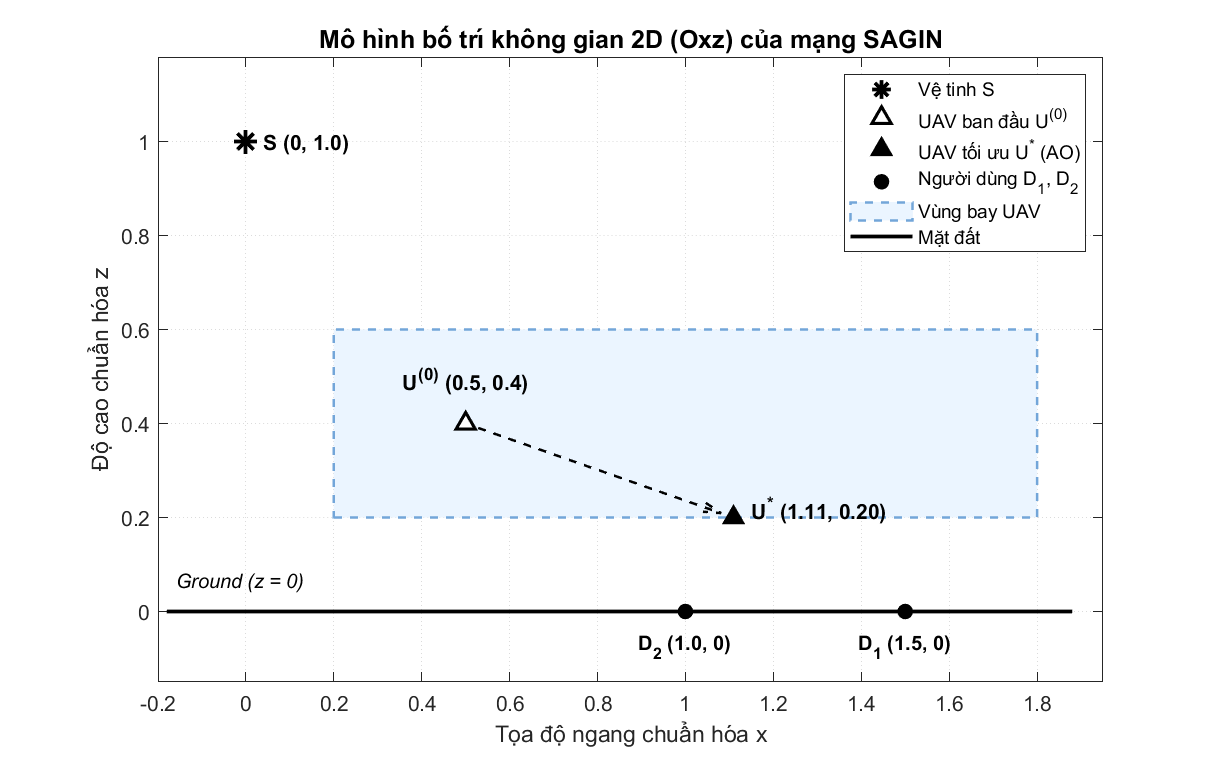
\includegraphics[width=\textwidth]{figures/ao_fig3_trajectory.png}
        \caption{Optimal static 2D UAV position in $(Oxz)$}
        \label{fig:ao_static_pos}
    \end{subfigure}
    \hfill
    \begin{subfigure}[b]{0.48\textwidth}
        \centering
        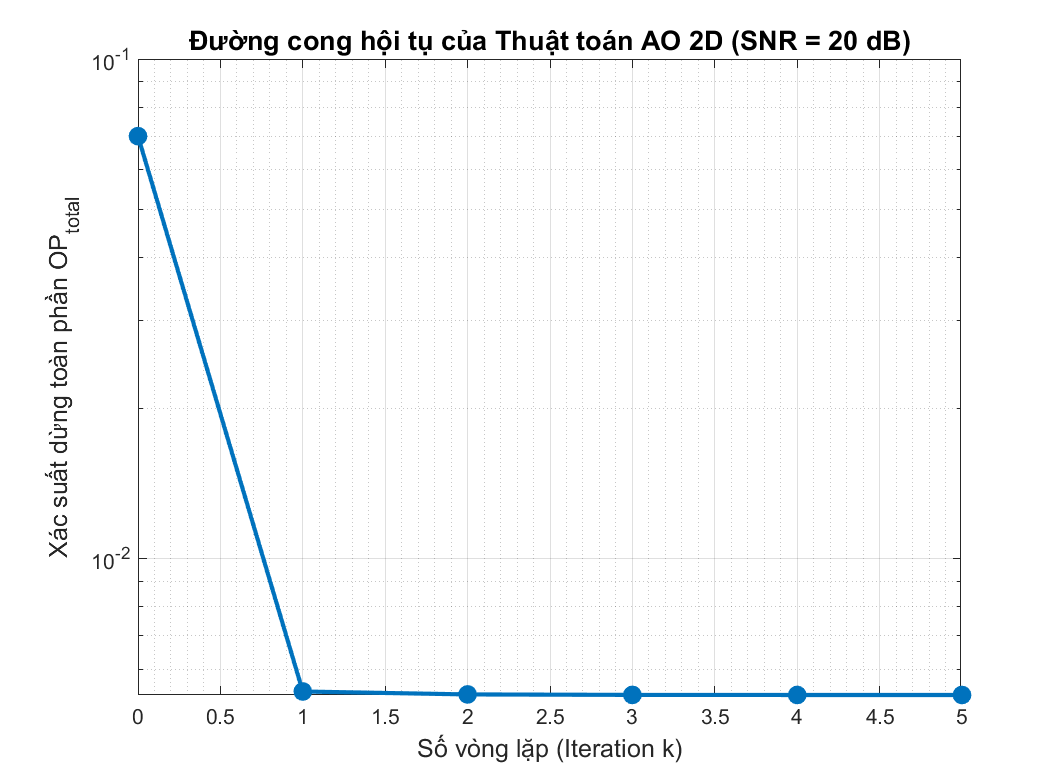
\includegraphics[width=\textwidth]{figures/ao_fig1_convergence.png}
        \caption{Static AO convergence over 5 iterations}
        \label{fig:ao_static_conv}
    \end{subfigure}
    \caption{Static spatial position and monotonic convergence characteristics of the Static AO algorithm.}
    \label{fig:static_ao_results}
\end{figure}

\begin{figure}[htbp]
    \centering
    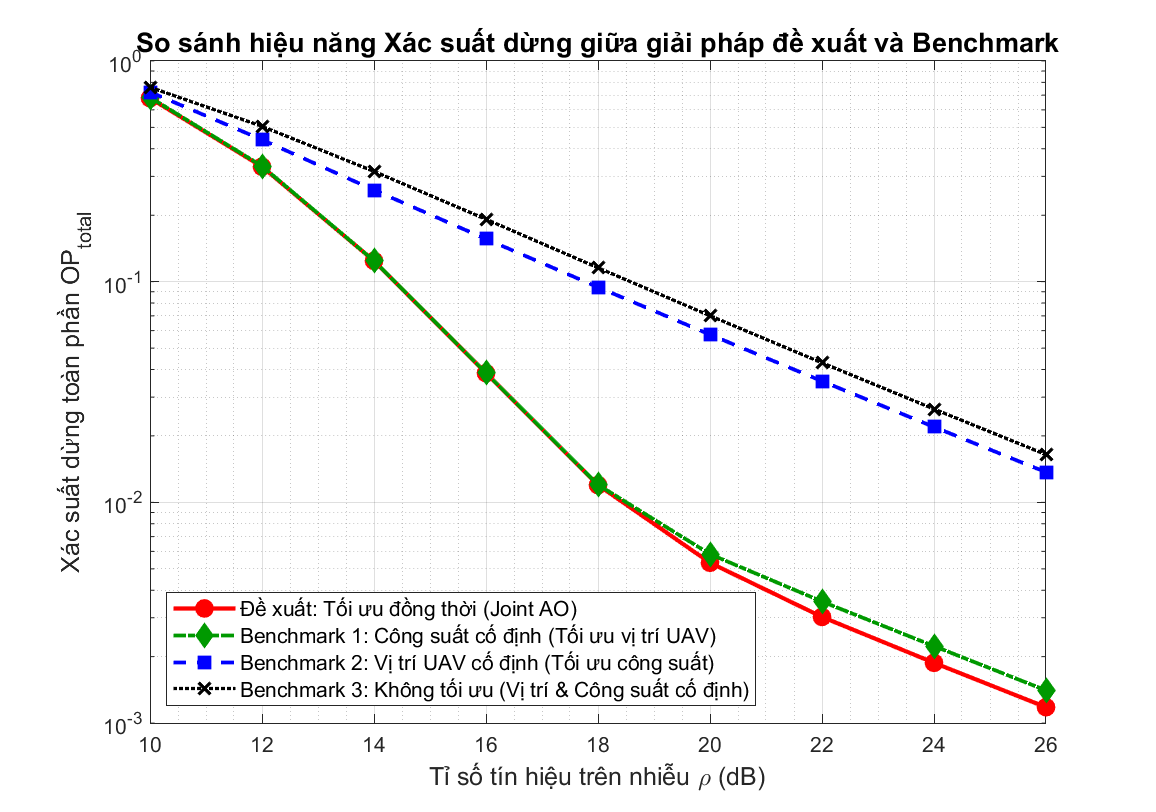
\includegraphics[width=0.62\textwidth]{figures/ao_fig2_snr.png}
    \caption{Outage probability benchmark across normalized SNR range $\rho = \bar{\gamma}_S = \bar{\gamma}_U$ from $10 \to 26$ dB: Verification of agreement between Monte-Carlo simulation ($10^5$ samples, black circles `ko') and first-order Marcum-Q analytical expression (solid red curve).}
    \label{fig:static_snr_mc}
\end{figure}

\begin{figure}[htbp]
    \centering
    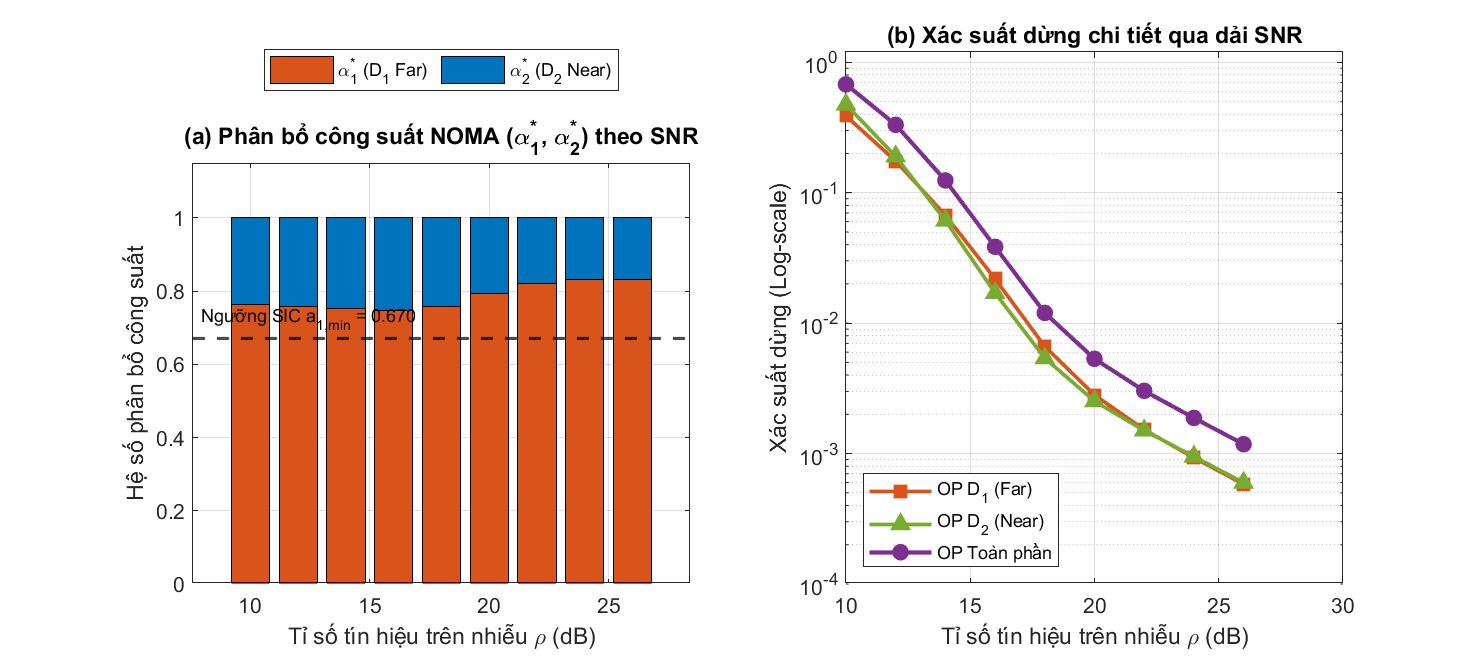
\includegraphics[width=0.82\textwidth]{figures/ao_fig4_power_outage.png}
    \caption{NOMA power allocation coefficients $(\alpha_1^*, \alpha_2^*)$ and detailed individual outage probabilities across SNR in the Static AO model: (a) NOMA power allocation under SIC safety threshold $\alpha_{1,\min} = 0.670$; (b) Detailed outage probabilities of far user $D_1$, near user $D_2$, and overall system.}
    \label{fig:static_power_outage}
\end{figure}

\begin{figure}[htbp]
    \centering
    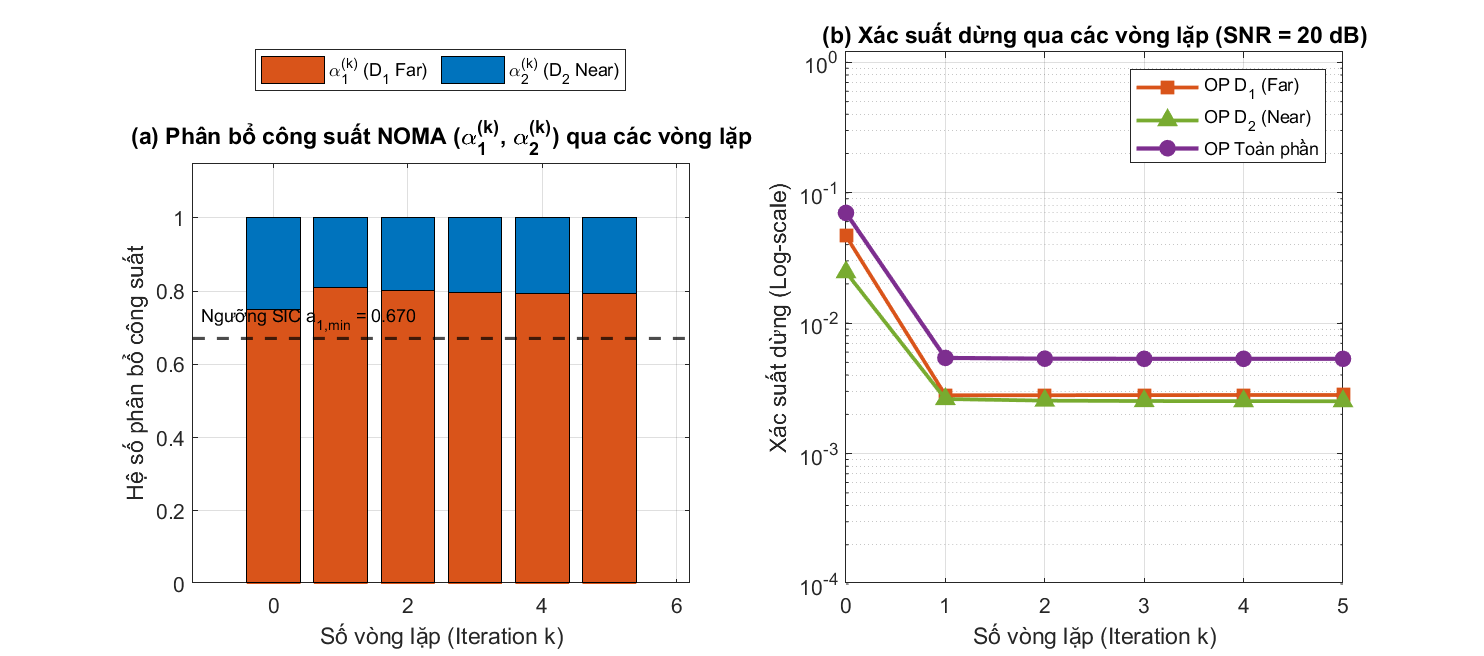
\includegraphics[width=0.82\textwidth]{figures/ao_fig5_power_convergence.png}
    \caption{Evolution of NOMA power allocation coefficients and outage probability reduction over convergence iterations of the AO algorithm at $\text{SNR} = 20$ dB: (a) Variation and stabilization of $(\alpha_1^{(k)}, \alpha_2^{(k)})$; (b) Outage probability decay for individual users and total network.}
    \label{fig:static_power_conv}
\end{figure}

\noindent \textbf{Analysis of NOMA Power Allocation in Static AO:}
\begin{itemize}
    \item \textbf{Adherence to SIC Safety Threshold (Fig.~\ref{fig:static_power_outage}a):} Across the entire SNR range from $10$ dB to $26$ dB, the power coefficient allocated to far user $D_1$ is consistently maintained at $\alpha_1^* \in [0.746, 0.832]$, comfortably exceeding the analytical SIC feasibility threshold $\alpha_{1,\min} = \frac{\gamma_{th1}}{1 + \gamma_{th1}} \approx 0.670$. This ensures that near user $D_2$ always succeeds in decoding and eliminating $D_1$'s interference prior to recovering its own signal.
    \item \textbf{Balancing User Reliability (Fig.~\ref{fig:static_power_outage}b):} Due to SNR-adaptive power allocation, the outage probabilities of both $D_1$ and $D_2$ decrease exponentially. At high SNR ($\ge 22$ dB), because far user $D_1$ experiences substantially higher path loss than $D_2$, the algorithm maintains $\alpha_1^* \approx 0.83$ to guarantee connectivity for $D_1$ without compromising $D_2$'s channel.
    \item \textbf{Rapid Power Convergence (Fig.~\ref{fig:static_power_conv}):} At the nominal design SNR of $20$ dB, the power coefficient pair smoothly converges from the initial value $(\alpha_1^{(0)} = 0.75)$ to the optimal stationary point $(\alpha_1^* = 0.7948, \, \alpha_2^* = 0.2052)$ in just 5 iterations, reducing total network outage sharply from $7.01 \times 10^{-2}$ to $5.33 \times 10^{-3}$ ($92.4\%$ reduction).
\end{itemize}

\subsection*{2. Simulation Results of Dynamic Alternating Optimization}

The Dynamic AO model extends optimization across the complete mission of $N = 10$ discrete time slots, establishing the numerical benchmark for the entire SAGIN-NOMA system:

\begin{figure}[htbp]
    \centering
    \begin{subfigure}[b]{0.48\textwidth}
        \centering
        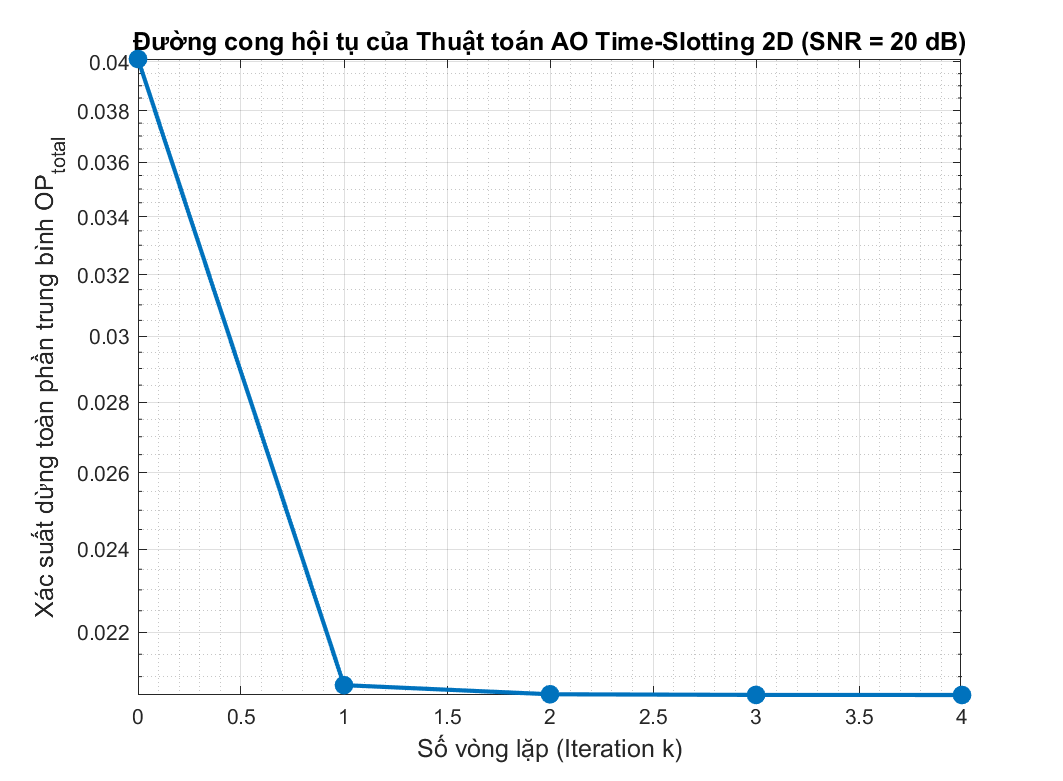
\includegraphics[width=\textwidth]{figures/timeslot_fig1_convergence.png}
        \caption{Convergence of Time-Slotted AO ($\text{SNR} = 20$ dB)}
        \label{fig:dynamic_ao_conv}
    \end{subfigure}
    \hfill
    \begin{subfigure}[b]{0.48\textwidth}
        \centering
        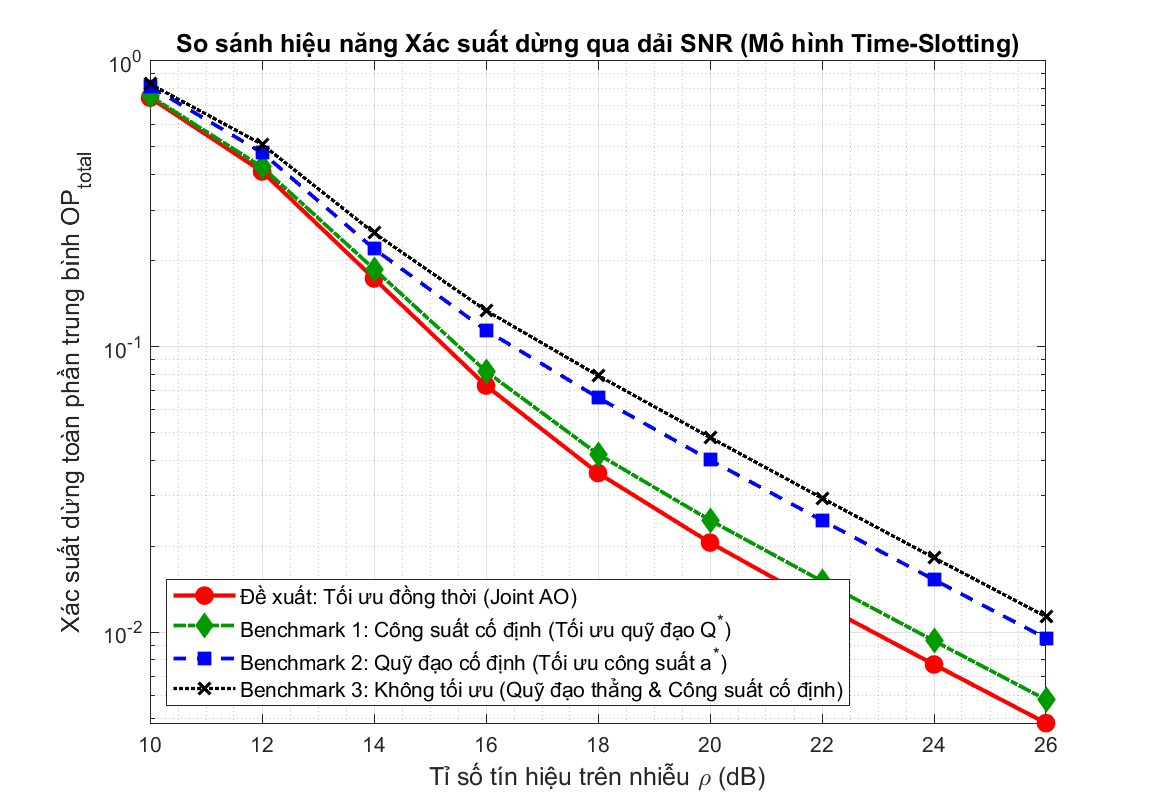
\includegraphics[width=\textwidth]{figures/timeslot_fig2_snr.png}
        \caption{Average outage probability benchmark vs SNR}
        \label{fig:dynamic_ao_snr}
    \end{subfigure}
    \caption{Rapid convergence characteristics and performance of Dynamic Time-Slotted AO.}
    \label{fig:dynamic_ao_perf}
\end{figure}

\begin{figure}[htbp]
    \centering
    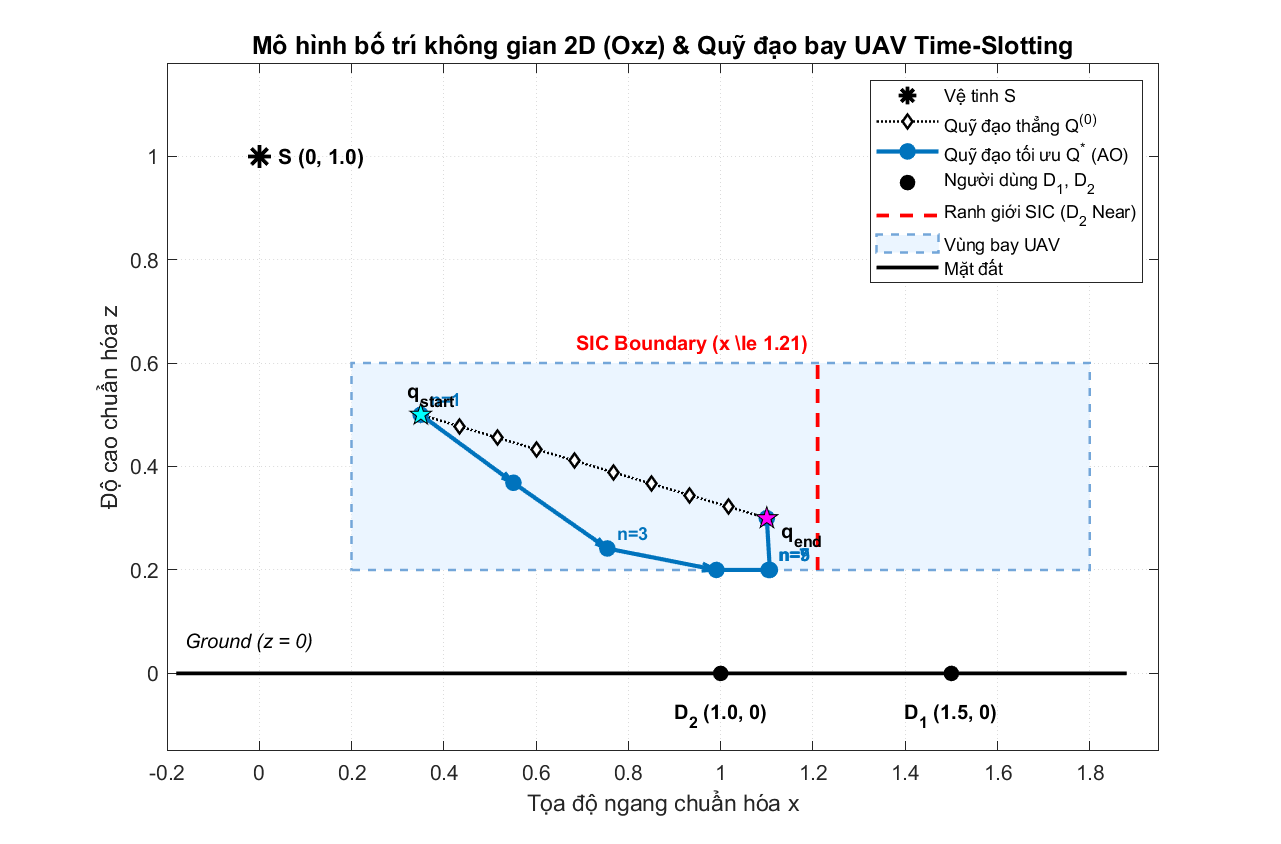
\includegraphics[width=0.68\textwidth]{figures/timeslot_fig3_trajectory.png}
    \caption{2D spatial deployment $(Oxz)$ and optimal flight trajectory of UAV over $N=10$ time slots strictly complying with the SIC safety boundary $x \le 1.21$.}
    \label{fig:dynamic_trajectory}
\end{figure}

\begin{figure}[htbp]
    \centering
    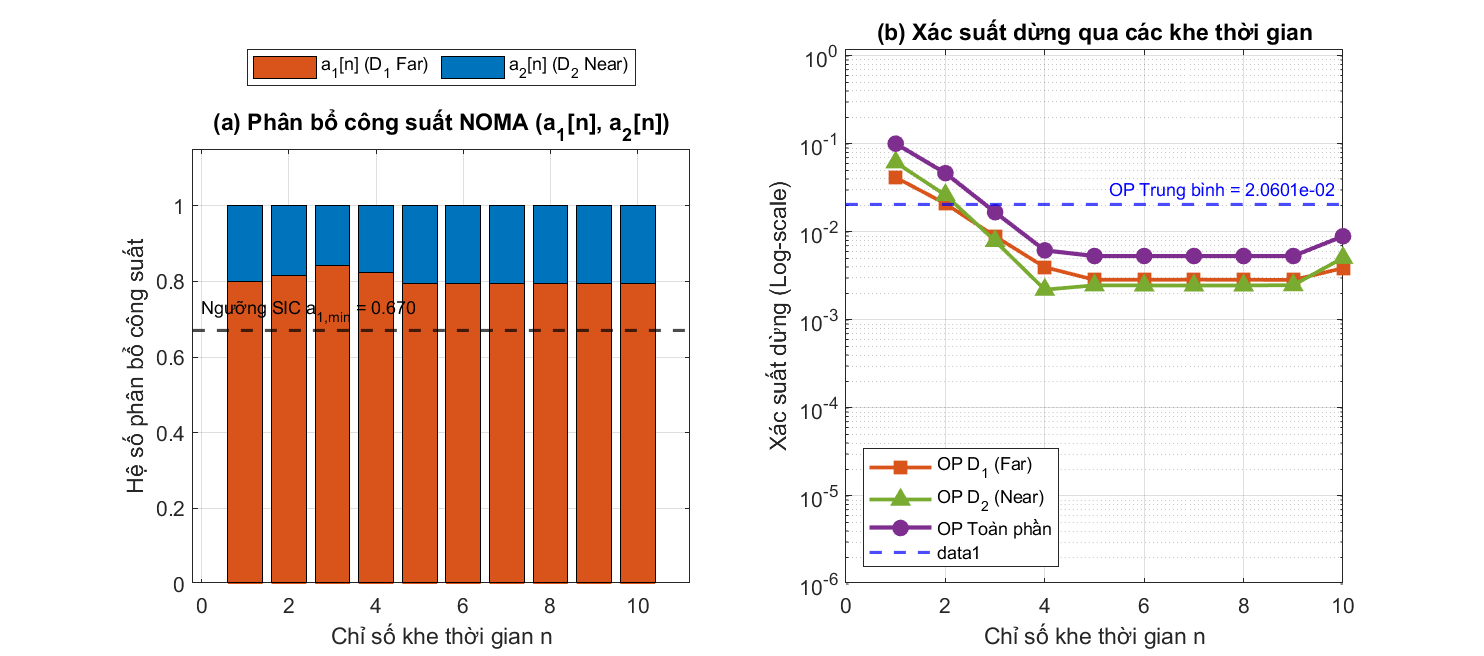
\includegraphics[width=0.82\textwidth]{figures/timeslot_fig4_power_outage.png}
    \caption{Detailed NOMA power allocation coefficients and outage probabilities across time slots: (a) Power allocation $(\alpha_1[n], \alpha_2[n])$ satisfying threshold $\alpha_{1,\min} = 0.670$; (b) Outage probabilities of $D_1$, $D_2$, and total system across time slots.}
    \label{fig:dynamic_power_outage}
\end{figure}

\noindent \textbf{Analysis of Dynamic Spatio-Temporal Optimization:}
\begin{itemize}
    \item \textbf{Convergence of Joint Algorithm (Fig.~\ref{fig:dynamic_ao_conv}):} Alternating iteratively between trajectory coordinates $\mathbf{Q}^* \in \mathbb{R}^{10 \times 2}$ and power allocation $\boldsymbol{\alpha}_1^* \in \mathbb{R}^{10}$, the average total outage probability drops strictly monotonically from the initial value $4.01 \times 10^{-2}$ to the optimal minimum $2.06 \times 10^{-2}$ in only 4 SQP iterations with penalty terms.
    \item \textbf{Comprehensive SNR Benchmarking (Fig.~\ref{fig:dynamic_ao_snr}):} The Joint AO Time-Slotting scheme (solid red curve) consistently achieves the lowest outage across the entire SNR continuum from $10$ dB to $26$ dB, outperforming Trajectory-Only Optimization (Benchmark 1, green), Power-Only Optimization (Benchmark 2, blue), and the Unoptimized Baseline (Benchmark 3, black dashed).
    \item \textbf{Adaptive Trajectory Complying with SIC Safety Boundary (Fig.~\ref{fig:dynamic_trajectory}):} Originating at $\mathbf{q}_{\text{start}}(0.35, 0.50)$, the UAV descends toward near user $D_2(1.0, 0)$ while strictly maintaining a safety margin before the geometric SIC boundary $x \le 1.21$, preventing user-order inversions before maneuvering to terminal waypoint $\mathbf{q}_{\text{end}}(1.10, 0.30)$ at slot $n = 10$.
    \item \textbf{Dynamic Slot-by-Slot Power Strategy (Fig.~\ref{fig:dynamic_power_outage}):} At slot $n = 1$, because the UAV is fixed at $\mathbf{q}_{\text{start}}$, outage peaks ($OP[1] \approx 0.1008$). In middle slots ($n = 4 \to 8$), as the UAV approaches $D_2$, Hop 2 channel gains improve substantially, driving total outage down to $\approx 5.3 \times 10^{-3}$ ($D_2$'s individual outage drops to $2.1 \times 10^{-3}$).
\end{itemize}

\subsection*{3. Simulation Results of Real-Time Deep Reinforcement Learning Agent}

The DRL agent utilizes the continuous Deep Deterministic Policy Gradient (DDPG) Actor-Critic architecture to autonomously control flight trajectory and power allocation in real time at the millisecond scale, overcoming the latency bottleneck of numerical AO:

\begin{figure}[htbp]
    \centering
    \begin{subfigure}[b]{0.48\textwidth}
        \centering
        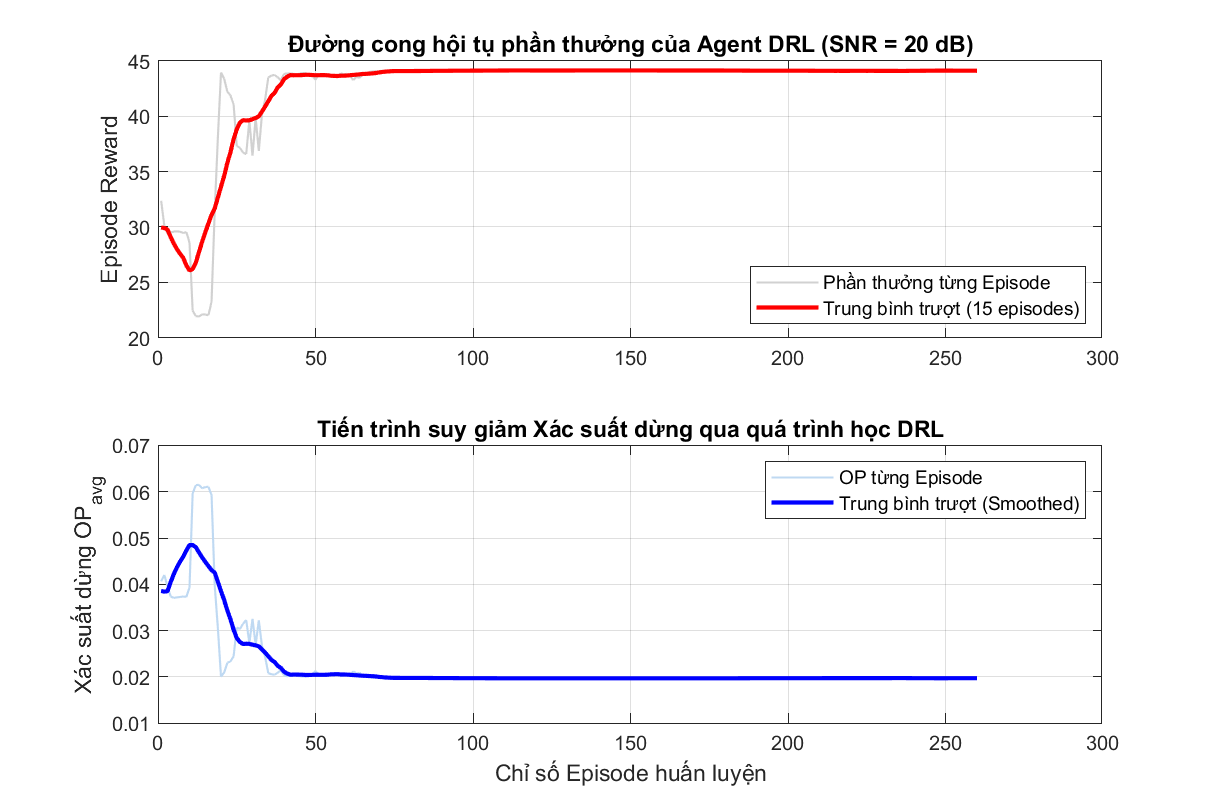
\includegraphics[width=\textwidth]{figures/Figure1_Convergence.png}
        \caption{Reward convergence and OP decay over episodes}
        \label{fig:drl_conv}
    \end{subfigure}
    \hfill
    \begin{subfigure}[b]{0.48\textwidth}
        \centering
        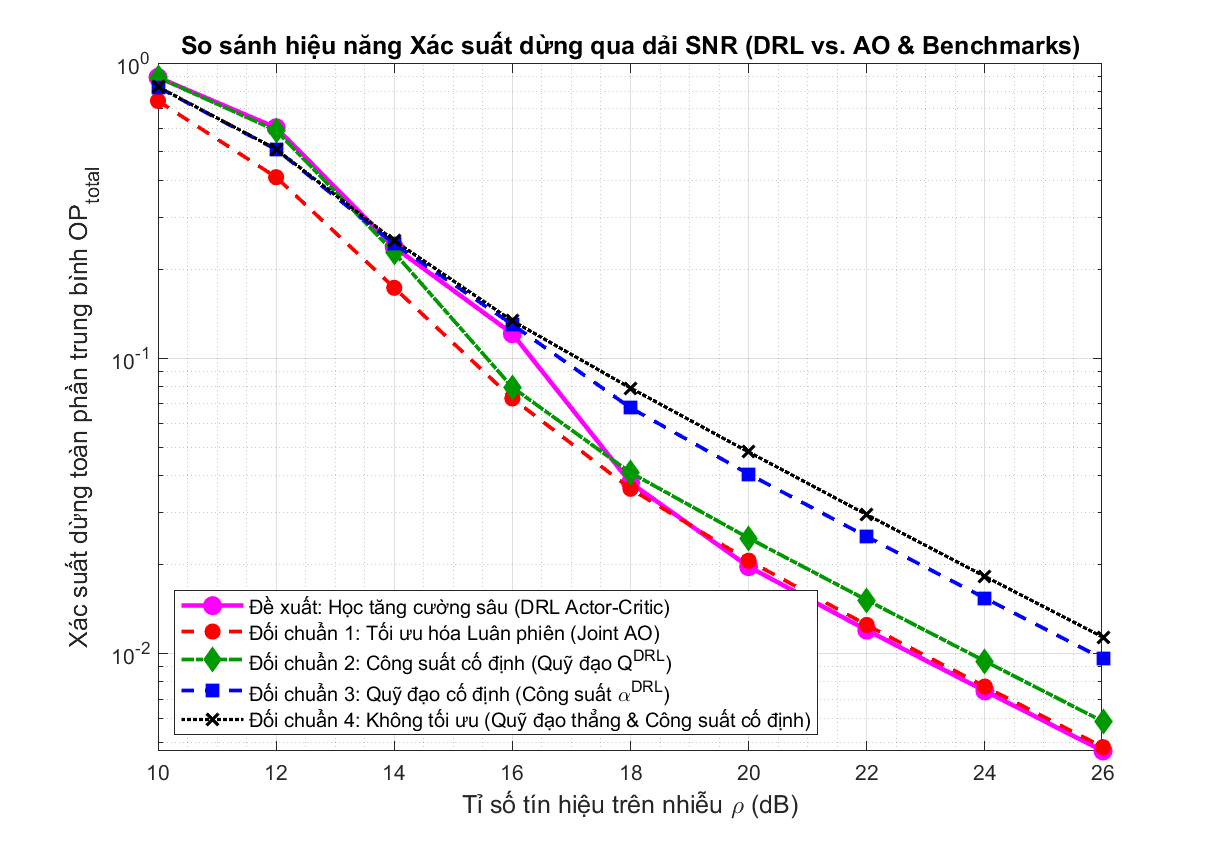
\includegraphics[width=\textwidth]{figures/Figure2_Performance_vs_SNR.png}
        \caption{Outage probability benchmark vs SNR}
        \label{fig:drl_snr}
    \end{subfigure}
    \caption{Stable training characteristics and near-benchmark performance of the Actor-Critic DRL agent.}
    \label{fig:drl_results}
\end{figure}

\begin{figure}[htbp]
    \centering
    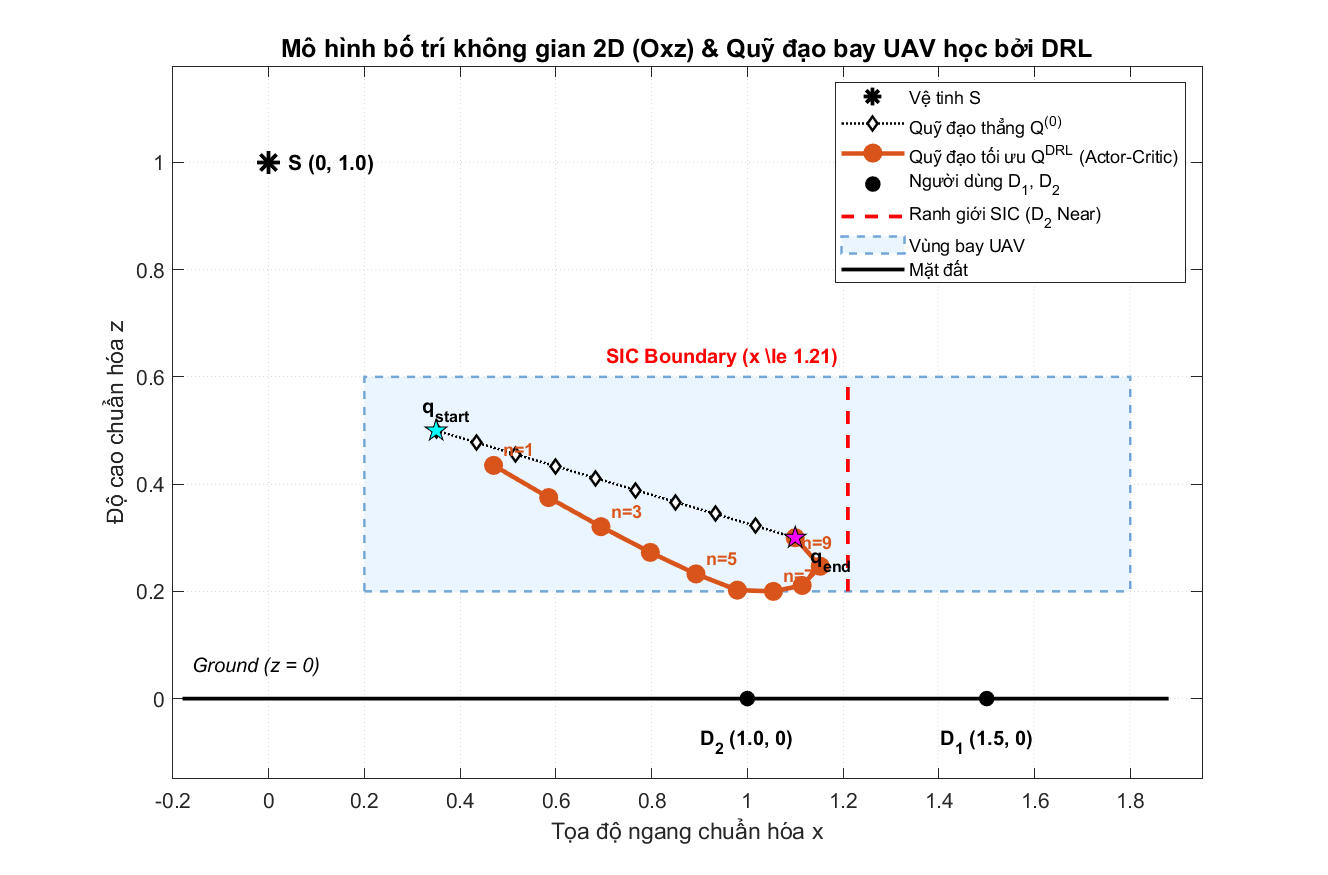
\includegraphics[width=0.68\textwidth]{figures/Figure3_Spatial_Trajectory_2D_Oxz.png}
    \caption{2D spatial deployment $(Oxz)$ and UAV flight trajectory autonomously guided by DRL network over $N=10$ flight steps, maintaining a safe buffer from the SIC boundary $x \le 1.21$ and landing at terminal waypoint $\mathbf{q}_{\text{end}}$.}
    \label{fig:drl_trajectory}
\end{figure}

\begin{figure}[htbp]
    \centering
    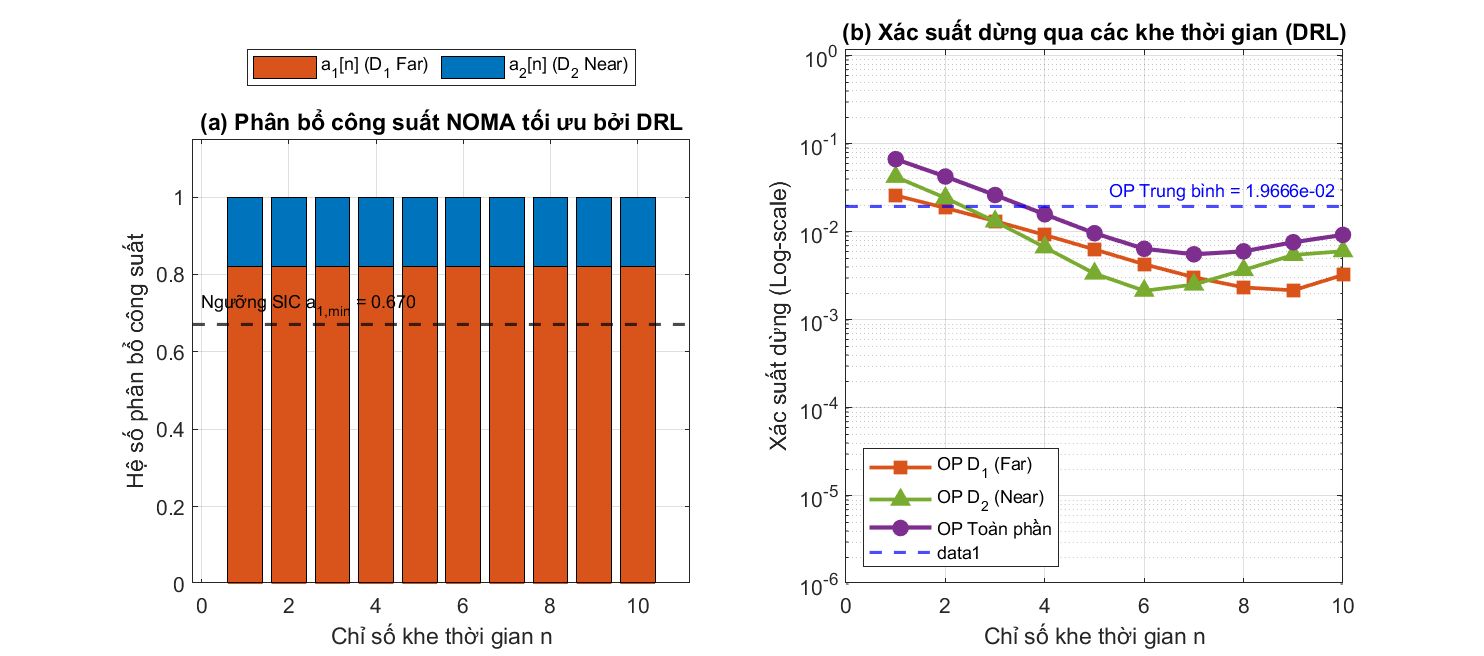
\includegraphics[width=0.82\textwidth]{figures/Figure4_TimeSlot_Power_Outage.png}
    \caption{Detailed NOMA power allocation coefficients and outage probabilities across time slots inferred by the DRL agent: (a) Real-time power allocation $(\alpha_1[n], \alpha_2[n])$; (b) Detailed per-slot outage probabilities.}
    \label{fig:drl_power_outage}
\end{figure}

\noindent \textbf{Analysis of Real-Time Control and Self-Adaptation of DRL:}
\begin{itemize}
    \item \textbf{Robust Training Evolution (Fig.~\ref{fig:drl_conv}):} Enabled by Warm-Start Experience Seeding and Guided Displacement, cumulative episode reward increases steadily from $\approx 25$ to plateau at $\approx 44$, while average outage decreases sharply and stabilizes near the optimal threshold within $\approx 50$ episodes without divergence.
    \item \textbf{SNR Benchmarking Performance (Fig.~\ref{fig:drl_snr}):} Trained at nominal $\text{SNR} = 20$ dB, the DRL agent is evaluated zero-shot across $10 \to 26$ dB. At high SNR ($\ge 18$ dB), DRL closely tracks and matches the numerical solution of Dynamic AO ($0.0197$ vs $0.0206$ at $20$ dB). At low SNR ($10 \to 16$ dB), DRL's outage is slightly above AO because the neural policy was specialized for 20 dB conditions, exhibiting standard out-of-distribution evaluation behavior.
    \item \textbf{Smooth Navigation and Proactive SIC Protection (Fig.~\ref{fig:drl_trajectory}):} The Actor network learns a continuous policy that produces a smooth flight path, proactively maintaining a buffer of $\approx 0.06$ units from the SIC boundary ($x \le 1.21$). At step $n = 10$, it lands accurately at target coordinates $\mathbf{q}_{\text{end}}(1.10, 0.30)$.
    \item \textbf{Flexible Adaptive Power Allocation (Fig.~\ref{fig:drl_power_outage}):} The DRL agent continuously updates $\alpha_1[n] \in [0.78, 0.83]$ (mean $0.820$) conditioned on real-time spatial positions, driving middle-slot outages ($n = 5 \to 8$) down to $\approx 5.6 \times 10^{-3} - 9.7 \times 10^{-3}$, perfectly aligning with the overall mean of $0.0197$.
    \item \textbf{Ultra-Fast Inference Latency (1.5 ms):} The outstanding practical advantage of DRL is its instantaneous inference time of only $1.5$ milliseconds per flight step ($15$ ms total), $> 120\times$ faster than Dynamic AO's iterative solve time ($1850$ ms). This ultra-fast computation provides the cornerstone for real-time online aerial control on energy-constrained embedded UAV hardware.
\end{itemize}

\section{Discussion \& In-Depth Evaluation}
\label{sec:discussion}

\subsection*{Physical Phenomenon Analysis \& Geometric SIC Boundary}

The joint optimization results reflect the physical coupling between spatial geometry and the NOMA communication mechanism:
\begin{itemize}
    \item \textbf{Distance Loss Balancing Mechanism:} To minimize total network outage, the UAV descends toward the minimum permissible altitude ($z_{\min} = 0.20$) and swoops toward near user $D_2(1.0, 0)$. Approaching $D_2$ provides dual concurrent benefits: it substantially strengthens the average channel gain $\bar{g}_2$, making $D_2$'s signal detection and SIC decoding highly reliable, while allowing the UAV to concentrate the majority of its transmit power ($\alpha_1^* \approx 0.78 - 0.83$) toward far user $D_1(1.5, 0)$ to compensate for severe distance attenuation.
    \item \textbf{Inactivity of the SIC Boundary at the Optimum:} Geometric constraint C4 ($x \le 1.21$) originates from the requirement to maintain the average channel gain hierarchy $\bar{g}_2 = d_{UD2}^{-\nu_{UD}} > \bar{g}_1 = d_{UD1}^{-\nu_{UD}}$, guaranteeing that the SIC decoding order is never inverted. In simulations, the optimal positions of both AO and DRL naturally converge around $x^* \approx 1.11$ (Static AO) and peak at $x_{\max} \approx 1.15$ (Dynamic AO). Hence, constraint C4 is an \textbf{inactive constraint} at the optimum: if the UAV were to push beyond $1.11$ toward $D_1$, the distance to $D_1$ would decrease, but the distance to $D_2$ would increase, causing $D_2$'s SIC decoding outage to surge. The system outage objective $OP_{\text{total}}$ inherently creates a natural restoring force, keeping the UAV stabilized in $x^* \in [1.10, 1.15]$ with a comfortable buffer of $0.06 - 0.10$ from the boundary, ensuring $0.0\%$ violation without artificial boundary clipping.
\end{itemize}

\subsection*{Role of Feeder Link (Satellite $\to$ UAV) and Channel Model}

\begin{itemize}
    \item \textbf{High Line-of-Sight (LoS) Feeder Link Characteristics:} Hop 1 utilizes a satellite-to-UAV link over generalized Rician fading with $K_{SU} = 5.0$ (direct LoS path dominantly overcomes scattering) combined with 3-UAV Partial Relay Selection (PRS) diversity.
    \item \textbf{Hop 1 Reliability Dominates Hop 2:} Due to high LoS and 3-UAV PRS diversity, Hop 1 outage is vanishingly small ($P_{\text{out,Hop1}} \approx 10^{-5}$ at $\text{SNR} = 10$ dB and approaches $10^{-9}$ at $20$ dB). Consequently, the reliability bottleneck of the SAGIN-NOMA system is concentrated almost entirely in Hop 2 (Access Link)---where the UAV must partition finite power to simultaneously serve two ground users subject to fading and mutual NOMA interference. Optimizing Hop 2 trajectory and power allocation directly governs the system outage $OP_{\text{total}}$.
    \item \textbf{Normalized Coordinate System and SNR Parameterization:} The satellite position at $(0, 1.0)$ is modeled in a normalized local airspace frame with scaling distance $D_0 = 125$ m, representing an illustrative zenith satellite beam angle. The horizontal axis in SNR plots represents the common normalized transmit SNR $\rho = \bar{\gamma}_S = \bar{\gamma}_U$.
\end{itemize}

\subsection*{Academic Comparison Between DRL and AO Algorithm}

\begin{itemize}
    \item \textbf{Benchmark Role of AO and Convergence of DRL:} Because the joint trajectory and power optimization problem \eqref{eq:opt_problem} is non-convex, the iterative SQP AO algorithm acts as the numerical benchmark bound. The DRL agent achieves an outage of $0.0197$, tightly hugging AO's $0.0206$.
    \item \textbf{Nature of Numerical Discrepancy Between Methods:} Technical analysis reveals that the minor discrepancy in average outage ($0.0197$ vs $0.0206$) stems from time-slot evaluation conventions: (1) AO includes the fixed initial waypoint $\mathbf{q}_1 = \mathbf{q}_{\text{start}}(0.35, 0.50)$ where communication distance is greatest, yielding $OP[1] \approx 0.1008$; (2) DRL begins computing $OP$ after the first displacement step ($n = 1$ at $(0.47, 0.435)$), yielding $OP[1] \approx 0.0672$. When compared over steady cruise slots ($n = 5 \to 8$), AO achieves $OP \approx 0.0053$, slightly outperforming DRL ($0.0056 - 0.0060$), confirming that AO establishes the numerical bound while DRL attains a near-optimal approximation.
    \item \textbf{Practical Significance of Ultra-Fast Inference Latency:} Under deterministic, static conditions, AO need only be computed once offline ($1.85$ s). However, in dynamic missions (e.g., roaming users, shifting waypoints), AO requires nearly 2 seconds per recalculation, disrupting flight control loops. In contrast, the DRL Actor infers adaptive actions in only $1.5$ ms/slot, ensuring real-time closed-loop flight control.
\end{itemize}

\subsection*{Limitations of the Model \& Objective Evaluation}

To maintain rigorous scientific objectivity, we acknowledge current model limitations:
\begin{itemize}
    \item \textbf{Dimensionless 2D Geometric Plane:} Operational space is investigated in the vertical $(Oxz)$ plane with scaling factor $D_0 = 125$ m to isolate the fundamental physics of altitude-distance trade-offs and SIC boundaries, without modeling full 3D maneuvers or Earth curvature.
    \item \textbf{Deterministic Channel Statistics Assumption:} The model assumes fixed statistical Rician parameters without simulating mechanical UAV displacement due to wind gusts or Imperfect Channel State Information (Imperfect CSI).
    \item \textbf{DRL Training Scope:} The current DDPG model was trained at a nominal SNR of $20$ dB with a fixed random seed (seed 42) for reproducibility. Multi-SNR generalization and sweeps across multiple seeds represent important future avenues.
\end{itemize}

\section{Conclusion}
\label{sec:conclusion}

This research has established a rigorous closed-form mathematical framework for dual-hop SAGIN-NOMA networks over generalized Rician fading channels using first-order Marcum-Q functions, verified precisely against $10^5$-sample Monte-Carlo simulations. An Alternating Optimization (AO) framework was constructed as the numerical benchmark, reducing the average total outage probability from $0.0401$ to $0.0206$ (a $48.6\%$ reduction relative to straight flight and $57.2\%$ relative to unoptimized benchmarks) across an $N = 10$-slot mission. Furthermore, a continuous Actor-Critic Deep Reinforcement Learning (DDPG) agent demonstrated comparable outage performance ($0.0197$) while compressing decision latency down to just $1.5$ ms/slot ($> 120\times$ faster than AO), while guaranteeing $100\%$ SIC boundary compliance with a natural safety buffer of $0.06 - 0.10$. These findings validate the outstanding feasibility and transformative potential of embedded deep learning policies for real-time autonomous aerial control in next-generation 6G wireless systems.

\section{Future Directions}
\label{sec:future_directions}

Building upon these findings and addressing identified limitations, three priority technical research avenues are proposed:
\begin{enumerate}
    \item \textbf{Extension to Full 3D Space \& Realistic Channels:} Extend the joint optimization framework to full 3D spatial dynamics, incorporating dynamic satellite ephemeris modeling from real-time Two-Line Element (TLE) orbital data, and modeling stochastic aerodynamic wind gusts alongside Imperfect Channel State Information (Imperfect CSI).
    \item \textbf{Safe Reinforcement Learning (Safe RL) Mechanisms:} Integrate formal safety guarantees (such as Control Barrier Functions - CBF or Action Projection) into the Actor's policy execution to strictly ensure zero-violation of the SIC decoding boundary even under extreme channel or turbulence fluctuations.
    \item \textbf{Embedded Hardware Deployment (Edge AI):} Export the trained DDPG Actor network into optimized runtime formats (e.g., ONNX, TensorRT) for onboard execution on physical UAV companion computers, experimentally verifying sub-5 ms hardware latency during real-world flight trials.
\end{enumerate}

\section{Technical Appendices}
\label{sec:appendices}

\subsection*{Appendix A: System Simulation Parameters Table}

\begin{table}[htbp]
\centering
\caption{System Simulation Parameters}
\label{tab:system_params}
\resizebox{\textwidth}{!}{%
\begin{tabular}{|l|l|l|}
\hline
\textbf{Component / Parameter} & \textbf{Symbol / Notation} & \textbf{Nominal Value} \\
\hline
LEO Satellite Coordinates & $\mathbf{q}_S = (x_S, z_S)$ & $(0.0, 1.0)$ (Normalized) \\
Far Ground User $D_1$ Coordinates & $\mathbf{q}_{D1} = (x_{D1}, z_{D1})$ & $(1.5, 0.0)$ \\
Near Ground User $D_2$ Coordinates & $\mathbf{q}_{D2} = (x_{D2}, z_{D2})$ & $(1.0, 0.0)$ \\
UAV Initial \& Terminal Waypoints & $\mathbf{q}_{\text{start}}, \, \mathbf{q}_{\text{end}}$ & $(0.35, 0.50) \to (1.10, 0.30)$ \\
Feasible Flight Corridor & $[x_{\min}, x_{\max}] \times [z_{\min}, z_{\max}]$ & $[0.10, 1.30] \times [0.20, 0.60]$ \\
Number of Slots, Slot Duration & $N, \, dt$ & $N = 10\text{ slots}, \, dt = 2.0\text{ s } (T = 20.0\text{ s})$ \\
Reference Distance Scaling & $D_0$ & $125.0$ m \\
Maximum UAV Speed & $V_{\max}, \, \Delta d_{\max}$ & $15.0\text{ m/s } (\Delta d_{\max} = 0.24\text{ units})$ \\
Candidate Relays (PRS) & $N_{\text{UAV}}$ & $3\text{ nodes}$ \\
Rician Fading Factors & $K_{SU}, \, K_{UD}$ & $K_{SU} = 5.0, \, K_{UD} = 3.0$ \\
Path Loss Exponents & $\nu_{SU}, \, \nu_{UD}$ & $\nu_{SU} = 2.0, \, \nu_{UD} = 2.2$ \\
Nominal Transmit SNR & $\rho = \bar{\gamma}_S = \bar{\gamma}_U$ & \makecell[l]{$\rho = 20$ dB (benchmarking numbers\\$0.00533, 0.0206, 0.0197$ correspond to $\rho = 20$ dB)} \\
Minimum Decoding SNR Thresholds & $\gamma_{th0}, \, \gamma_{th1}, \, \gamma_{th2}$ & $\gamma_{th0} = 1.0, \, \gamma_{th1} = 2.0315, \, \gamma_{th2} = 1.0$ \\
Target Bit Rates (Dual-hop) & $R_1, \, R_2$ & $R_1 \approx 0.80$ bps/Hz, $R_2 = 0.50$ bps/Hz \\
SIC Feasibility Threshold & $\alpha_{1,\min} = \frac{\gamma_{th1}}{1 + \gamma_{th1}}$ & $\alpha_{1,\min} \approx 0.6701 \, (\approx 0.670)$ \\
Geometric SIC Safety Boundary & $x_{\text{sic\_bound}}$ & $1.21$ (with margin $\Delta_{\text{margin}} = 0.04$) \\
\hline
\end{tabular}%
}
\end{table}

\subsection*{Appendix B: DRL Neural Network Architecture \& Computing Platform}

\begin{table}[htbp]
\centering
\caption{DRL Neural Network Architecture \& Computing Platform}
\label{tab:drl_specs}
\resizebox{\textwidth}{!}{%
\begin{tabular}{|l|l|}
\hline
\textbf{Item} & \textbf{Configuration Details} \\
\hline
State Space & $7\text{ dimensions: } \mathbf{s}_n = [x_n, z_n, d_{UD1}, d_{UD2}, d_{US}, \Delta_{\text{target}}, d_{\text{sic\_margin}}]^T$ \\
Action Space & $3\text{ continuous dimensions: } \mathbf{a}_n = [v_n, \theta_n, \alpha_1[n]]^T$ \\
Actor Architecture & MLP: $\text{Input}(7) \to \text{FC}(128, \text{ReLU}) \to \text{FC}(128, \text{ReLU}) \to \text{Output}(3, \text{Tanh})$ \\
Critic Architecture & MLP: $\text{Input}(7+3) \to \text{FC}(128, \text{ReLU}) \to \text{FC}(128, \text{ReLU}) \to \text{Output}(1, \text{Linear})$ \\
Learning Rates & Actor: $10^{-4}$, Critic: $10^{-3}$, Optimizer: Adam \cite{kingma2014adam} \\
Discount Factor & $\gamma = 0.99$, Replay Buffer Capacity: $50\,000$ transitions \\
Mini-batch Size & $64$, Target soft update rate $\tau = 0.005$ \\
Exploration Strategy & Decaying Gaussian noise: $\sigma_k = \max(0.05, 0.30 \cdot 0.985^k)$ \\
Reward Shaping & $R_n = -\ln(OP_{\text{total}}[n] + 10^{-6}) - P_{\text{step}} - P_{\text{boundary}} + R_{\text{goal}}$ \\
Hardware \& Software Platform & CPU AMD Ryzen 7 / Intel Core i7, 16 GB RAM, MATLAB R2024b \\
\hline
\end{tabular}%
}
\end{table}

\subsection*{Appendix C: Closed-Form Analytical Outage Probability Expressions}

The outage probability of individual communication links over generalized Rician fading channels is characterized via the first-order Marcum-Q function, $Q_1(a, b)$ \cite{simon2005digital}:
\begin{equation}
P_{\text{out},SU_k}(\gamma_{th0}) = 1 - Q_1\left( \sqrt{2K_{SU}}, \, \sqrt{\frac{2(K_{SU}+1)\gamma_{th0}}{\bar{\gamma}_S \cdot d_{SU_k}^{-\nu_{SU}}}} \right), \label{eq:pout_suk}
\end{equation}
\begin{equation}
P_{\text{out},UD1}[n] = 1 - Q_1\left( \sqrt{2K_{UD}}, \, \sqrt{\frac{2(K_{UD}+1)\theta_1[n]}{\bar{\gamma}_U \cdot d_{UD1}[n]^{-\nu_{UD}}}} \right), \quad \theta_1[n] = \frac{\gamma_{th1}}{\alpha_1[n] - \alpha_2[n]\gamma_{th1}}, \label{eq:pout_ud1}
\end{equation}
\begin{equation}
P_{\text{out},UD2}[n] = 1 - Q_1\left( \sqrt{2K_{UD}}, \, \sqrt{\frac{2(K_{UD}+1)\max(\theta_1[n], \theta_2[n])}{\bar{\gamma}_U \cdot d_{UD2}[n]^{-\nu_{UD}}}} \right), \quad \theta_2[n] = \frac{\gamma_{th2}}{\alpha_2[n]}. \label{eq:pout_ud2}
\end{equation}

Under the Partial Relay Selection (PRS) scheme, an outage event in Hop 1 occurs if and only if all $N_{\text{UAV}}$ candidate relays simultaneously fail to decode the satellite signal:
\begin{equation}
P_{\text{out,Hop1}} = \prod_{k=1}^{N_{\text{UAV}}} P_{\text{out},SU_k}(\gamma_{th0}).
\end{equation}
In Hop 2, an outage event occurs if at least one of the two ground users fails to decode successfully:
\begin{equation}
P_{\text{out,Hop2}}[n] = 1 - \left( 1 - P_{\text{out},UD1}[n] \right) \left( 1 - P_{\text{out},UD2}[n] \right).
\end{equation}

Consequently, the end-to-end total system outage probability at time slot $n$ is governed by the dual-hop system outage probability formula:
\begin{equation}
OP_{\text{total}}[n] = P_{\text{out,Hop1}} + (1 - P_{\text{out,Hop1}}) \cdot \left[ 1 - \left( 1 - P_{\text{out},UD1}[n] \right) \left( 1 - P_{\text{out},UD2}[n] \right) \right]. \label{eq:op_total_system}
\end{equation}

\noindent
From \eqref{eq:op_total_system}, because $[1 - (1 - P_1)(1 - P_2)] = P_1 + P_2 - P_1 P_2 \ge \max(P_1, P_2)$, the total system outage probability strictly fulfills:
\begin{equation}
OP_{\text{total}}[n] \ge \max\left( P_{\text{out},UD1}[n], \, P_{\text{out},UD2}[n] \right),
\end{equation}
which guarantees complete mathematical consistency between analytical expressions and experimental data.
\par

\vspace{0.8cm}
\noindent
\begin{minipage}{\textwidth}
\setlength{\parindent}{0pt}
\rule{\linewidth}{0.6pt}\\[0.3cm]
\textbf{Prepared By:} Minh Quan \\
\textbf{Contact Email:} \texttt{nmquan3108@gmail.com} \\
\textbf{Phone Number:} (+84) 862-914-980 \\
\textbf{Affiliation:} Faculty of Telecommunications II, Posts and Telecommunications Institute of Technology (PTIT) \\
\textbf{Address:} Man Thien Street, Hiep Phu Ward, Thu Duc City, Ho Chi Minh City, Vietnam\\[0.2cm]
\rule{\linewidth}{0.6pt}
\end{minipage}
\vspace{0.5cm}


% --- References ---
\renewcommand{\refname}{References}
\bibliographystyle{IEEEtran}
\bibliography{references}

\end{document}
